\documentclass{beamer}
\mode<presentation>
\usepackage{amsmath}
\usepackage{amssymb}
%\usepackage{advdate}
\usepackage{adjustbox}
\usepackage{subcaption}
\usepackage{enumitem}
\usepackage{multicol}
\usepackage{mathtools}
\usepackage{listings}
\usepackage{url}
\def\UrlBreaks{\do\/\do-}
\usetheme{Boadilla}
\usecolortheme{lily}
% \setbeamertemplate{footline}
% {
%   \leavevmode%
%   \hbox{%
%   \begin{beamercolorbox}[wd=\paperwidth,ht=2.25ex,dp=1ex,right]{author in head/foot}%
%     \insertframenumber{} / \inserttotalframenumber\hspace*{2ex} 
%   \end{beamercolorbox}}%
%   \vskip0pt%
% }
\setbeamertemplate{navigation symbols}{}

\providecommand{\nCr}[2]{\,^{#1}C_{#2}} % nCr
\providecommand{\nPr}[2]{\,^{#1}P_{#2}} % nPr
\providecommand{\mbf}{\mathbf}
\providecommand{\pr}[1]{\ensuremath{\Pr\left(#1\right)}}
\providecommand{\qfunc}[1]{\ensuremath{Q\left(#1\right)}}
\providecommand{\sbrak}[1]{\ensuremath{{}\left[#1\right]}}
\providecommand{\lsbrak}[1]{\ensuremath{{}\left[#1\right.}}
\providecommand{\rsbrak}[1]{\ensuremath{{}\left.#1\right]}}
\providecommand{\brak}[1]{\ensuremath{\left(#1\right)}}
\providecommand{\lbrak}[1]{\ensuremath{\left(#1\right.}}
\providecommand{\rbrak}[1]{\ensuremath{\left.#1\right)}}
\providecommand{\cbrak}[1]{\ensuremath{\left\{#1\right\}}}
\providecommand{\lcbrak}[1]{\ensuremath{\left\{#1\right.}}
\providecommand{\rcbrak}[1]{\ensuremath{\left.#1\right\}}}
\theoremstyle{remark}
\newtheorem{rem}{Remark}
\newcommand{\sgn}{\mathop{\mathrm{sgn}}}
\providecommand{\abs}[1]{\left\vert#1\right\vert}
\providecommand{\res}[1]{\Res\displaylimits_{#1}} 
\providecommand{\norm}[1]{\lVert#1\rVert}
\providecommand{\mtx}[1]{\mathbf{#1}}
\providecommand{\mean}[1]{E\left[ #1 \right]}
\providecommand{\fourier}{\overset{\mathcal{F}}{ \rightleftharpoons}}
%\providecommand{\hilbert}{\overset{\mathcal{H}}{ \rightleftharpoons}}
\providecommand{\system}{\overset{\mathcal{H}}{ \longleftrightarrow}}
	%\newcommand{\solution}[2]{\textbf{Solution:}{#1}}
%\newcommand{\solution}{\noindent \textbf{Solution: }}
\providecommand{\dec}[2]{\ensuremath{\overset{#1}{\underset{#2}{\gtrless}}}}
\newcommand{\myvec}[1]{\ensuremath{\begin{pmatrix}#1\end{pmatrix}}}
\let\vec\mathbf

\lstset{
%language=C,
frame=single, 
breaklines=true,
columns=fullflexible
}

\numberwithin{equation}{section}

\title[MatGeo 3-3.3-2]{MatGeo Question 3-3.3-2}
\author[Shiven Bajpai]{Shiven Bajpai}
\institute[AI24BTECH11030]{AI24BTECH11030\\IIT Hyderabad}

\date{\today} 
\begin{document}

\begin{frame}
\titlepage
\end{frame}

\section*{Outline}
\begin{frame}
\tableofcontents
\end{frame}

\section{Problem}
\begin{frame}
\frametitle{Problem Statement}
Construct a triangle with sides $5cm$, $6cm$ and $7cm$
\end{frame}

\section{Solution}
\subsection{Calculating Cosine}
\begin{frame}
\frametitle{Calculating Cosine}

Let the vertices of triangle be $\vec{A}$, $\vec{B}$ and $\vec{C}$ and lengths of the sides opposing them be denoted by $a = 5cm$, $b = 6cm$ and $c = 7cm$ respectively.
\\

By Cosine rule in $\Delta ABC$,
\begin{align}
	a^2 &= b^2 + c^2 - 2bc \cos A\\
	\cos A &= \frac{b^2 + c^2 - a^2}{2bc}\\
	\label{eq:cosine} \cos A &= \frac{60}{84} 
\end{align}

\end{frame}

\subsection{Solving for points}
\begin{frame}[fragile]
\frametitle{Solving for points}

Let 
$$\vec{A} = \vec{0} \ \text{and} \ \vec{C} = \myvec{b \\ 0}$$
Then 
$$\vec{B} = c\myvec{\cos A \\ \sin A}$$

Substituting values from \ref{eq:cosine} we get, 
$$\vec{A} = \vec{0}, \ \vec{B} = \myvec{5 \\ \sqrt{24}}, \ \vec{C} = \myvec{6 \\ 0}$$
% The code in 
% {\footnotesize
% \begin{lstlisting}
% https://github.com/shivenBajpai/EE1030/blob/main/Question_6/Codes/main.py
% \end{lstlisting}
% }
% verifies the solution and provides the plot above
\end{frame}

\subsection{Code}
\begin{frame}[fragile, allowframebreaks]
	\frametitle{Code}
	This code can be found at
	{\footnotesize
	\begin{lstlisting}
https://github.com/shivenBajpai/EE1030/blob/main/Question_6/Codes/main.c
https://github.com/shivenBajpai/EE1030/blob/main/Question_6/Codes/main.py
	\end{lstlisting}
	}

	\lstset{
		language=C,
		basicstyle=\ttfamily\small,
		keywordstyle=\color{blue},
		stringstyle=\color{brown},
		commentstyle=\color{gray},
		tabsize=4
	}
	\lstinputlisting{Codes/main.c}

	\lstset{
		language=Python,
		basicstyle=\ttfamily\small,
		keywordstyle=\color{blue},
		stringstyle=\color{brown},
		commentstyle=\color{gray},
		tabsize=4
	}
	\lstinputlisting{Codes/main.py}
	
\end{frame}


\subsection{Plot}
\begin{frame}[fragile]
	\frametitle{Plot}

	\begin{figure}[H]
		\centering
		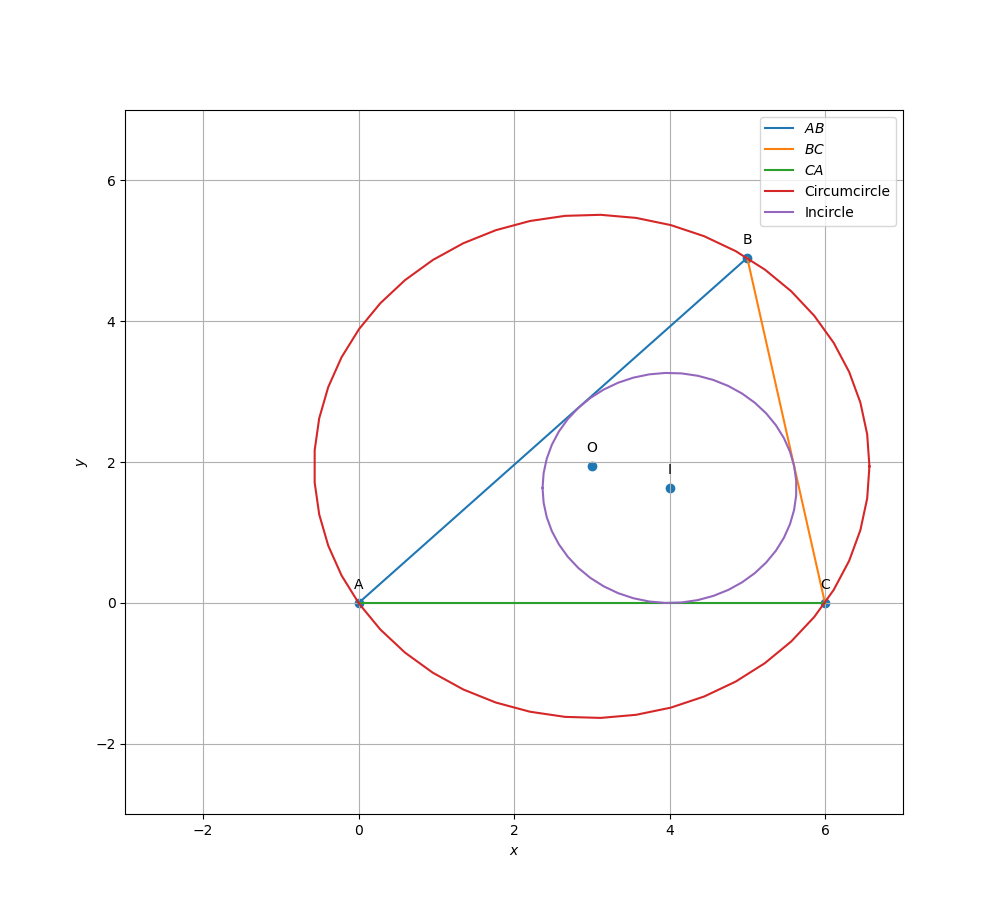
\includegraphics[width=0.675\textwidth]{figs/Figure.png}
	\end{figure}
	
	{\footnotesize
	\textsubscript{(Mihir asked me to plot the circles of the triangle)}}
\end{frame}

\section{Bonus: Alternate Approach}
\begin{frame}
\frametitle{Bonus Problem: Alternate Method}
Do it via intersection of circles, using matrices
\end{frame}

\subsection{Equations}
\begin{frame}
\frametitle{Equations}
	Let the vertices of triangle be $\vec{A}$, $\vec{B}$ and $\vec{C}$ and lengths of the sides opposing them be denoted by $a = 5cm$, $b = 6cm$ and $c = 7cm$ respectively.

	Let $\vec{A} = \vec{0}$ and $\vec{C} = \myvec{b \\ 0}$, then $\vec{B}$ satisfies

	\begin{align*}
		\Vert \vec{x} - \vec{A} \Vert &= c\\
		\Vert \vec{x} - \vec{C} \Vert &= a
	\end{align*}

	Since a point that lies on 2 circles lies on their radical axis, $\vec{B}$ lies on the line

	\begin{align*}
		\Vert \vec{x}\Vert^2 - 2\vec{C}^\text{T}\vec{x} + b^2 - a^2 &= \Vert \vec{x}\Vert^2 - 2\vec{A}^\text{T}\vec{x} - c^2 \\
		(\vec{C}-\vec{A})^\text{T}\vec{x} &= \frac{b^2 + c^2 - a^2}{2}
	\end{align*}
\end{frame}

\subsection{Solving Intersection}
\begin{frame}
\frametitle{Solving Intersection}
	Let $\vec{n} = (\vec{C} - \vec{A})$ and $d = \frac{b^2 + c^2 - a^2}{2}$

	Let parametric form of line be $\vec{x} = \vec{h} + k\vec{m}$

	Where $\vec{h} = \frac{\vec{n}d}{\Vert \vec{n} \Vert^2}$ and $\vec{m}$ be perpendicular to $\vec{n}$ i.e $\vec{m} = \myvec{-\vec{n}_2 \\ \vec{n}_1}$
	\\

	Substituting $\vec{x}$ in equation of circle
	\begin{align*}
		(\vec{h} + k\vec{m} - \vec{A})^\text{T} (\vec{h} + \vec{k}m - \vec{A}) &= c^2\\
		((\vec{h} - \vec{A}) + k\vec{m})^\text{T} ((\vec{h} - \vec{A}) + k\vec{m}) &= c^2\\
		(\vec{h} - \vec{A})^\text{T}(\vec{h} - \vec{A}) + 2k\vec{m}^\text{T}(\vec{h} - \vec{A}) + k^2\vec{m}^\text{T}\vec{m} &= c^2
	\end{align*}

	\text{Since $\vec{m}^T\vec{h} = 0$}
	\begin{align*}
		(\vec{h} - \vec{A})^\text{T}(\vec{h} - \vec{A}) - 2k\vec{m}^\text{T}\vec{A} + k^2\vec{m}^\text{T}\vec{m} &= c^2	
	\end{align*}
\end{frame}

\subsection{Solving for K}
\begin{frame}
\frametitle{Solving for K}

	Using quadratic formula for k,

	$$k = \frac{2\vec{m}^\text{T}\vec{A} \pm \sqrt{4(\vec{m}^\text{T}\vec{A})^2 - 4 (\vec{m}^\text{T}\vec{m})((\vec{h} - \vec{A})^\text{T}(\vec{h} - \vec{A}) - c^2)}}{2\vec{m}^\text{T}\vec{m}}$$

	$$k = \frac{\vec{m}^\text{T}\vec{A} \pm \sqrt{(\vec{m}^\text{T}\vec{A})^2 - (\vec{m}^\text{T}\vec{m})((\vec{h} - \vec{A})^\text{T}(\vec{h} - \vec{A}) - c^2)}}{\vec{m}^\text{T}\vec{m}}$$

	Since we have assumed $\vec{A} = \vec{0}$, We can simplify this to

	$$k = \frac{\pm \sqrt{(c^2 - \vec{h}^\text{T}\vec{h})}}{\sqrt{\vec{m}^\text{T}\vec{m}}}$$

	Then $\vec{x}$ is

	$$\vec{x} = \vec{h} \pm \frac{\sqrt{c^2 - \Vert \vec{h} \Vert^2} \; \vec{m}}{\Vert \vec{m} \Vert}$$
	
\end{frame}

\subsection{Solution}
\begin{frame}[fragile]
\frametitle{Solution}

Now substituting data,

\begin{align*}
	d &= 30\\
	\vec{h} &= \myvec{5 \\ 0}\\
	\vec{m} &= \myvec{0 \\ 6}\\
	k &= \pm \frac{\sqrt{24}}{6}\\
	\vec{B} &= \myvec{5 \\ \pm \sqrt{24}}
\end{align*}	

\end{frame}

\subsection{Code}
\begin{frame}[fragile, allowframebreaks]
	\frametitle{Code}
	This code can be found at
	{\footnotesize
	\begin{lstlisting}
https://github.com/shivenBajpai/EE1030/blob/main/Question_6/Codes/alt.c
https://github.com/shivenBajpai/EE1030/blob/main/Question_6/Codes/alt.py
	\end{lstlisting}
	}

	\lstset{
		language=C,
		basicstyle=\ttfamily\small,
		keywordstyle=\color{blue},
		stringstyle=\color{brown},
		commentstyle=\color{gray},
		tabsize=4
	}
	\lstinputlisting{Codes/alt.c}

	\lstset{
		language=Python,
		basicstyle=\ttfamily\small,
		keywordstyle=\color{blue},
		stringstyle=\color{brown},
		commentstyle=\color{gray},
		tabsize=4
	}
	\lstinputlisting{Codes/alt.py}
	
\end{frame}

\subsection{Plot}
\begin{frame}[fragile]
	\frametitle{Plot}

	\begin{figure}[H]
		\centering
		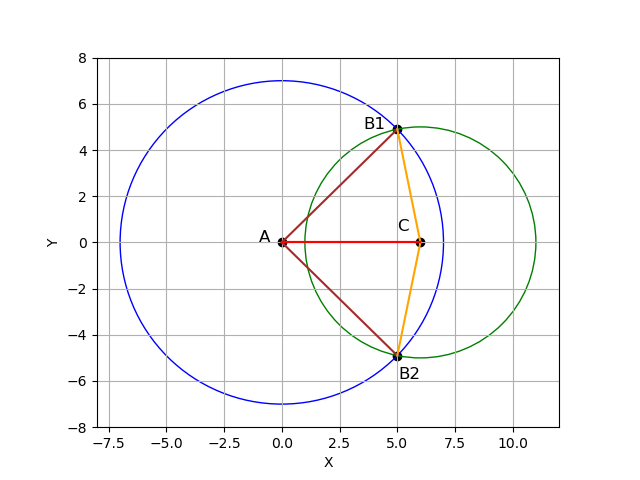
\includegraphics[width=0.75\textwidth]{figs/Alt_Figure.png}
	\end{figure}
\end{frame}

\end{document}